\documentclass[12pt]{article}

% Packages
\usepackage[margin=1in]{geometry}
\usepackage{amsmath, amsthm, amssymb}

\usepackage{graphicx}
\usepackage{listings}
\usepackage{xcolor}
\definecolor{codegreen}{rgb}{0,0.6,0}
\definecolor{codegray}{rgb}{0.5,0.5,0.5}
\definecolor{codepurple}{rgb}{0.58,0,0.82}
\definecolor{backcolour}{rgb}{0.95,0.95,0.92}
\lstset{
    backgroundcolor=\color{backcolour},   
    keywordstyle=\color{magenta},
    basicstyle=\ttfamily\footnotesize,
    breakatwhitespace=false,         
    breaklines=true,                 
    captionpos=b,                    
    keepspaces=true,                 
    showspaces=false,                
    showstringspaces=false,
    showtabs=false,                  
    tabsize=2
}

% Problem Box
\setlength{\fboxsep}{4pt}
\newsavebox{\mybox}
\newenvironment{problem}
    {\begin{lrbox}{\mybox}\begin{minipage}{0.98\textwidth}}
    {\end{minipage}\end{lrbox}\framebox[\textwidth]{\usebox{\mybox}}}

% Options
\renewcommand{\thesubsection}{\thesection(\alph{subsection})}
\allowdisplaybreaks
\addtolength{\jot}{1em}

% Default Commands
\newtheorem{proposition}{Proposition}
\newtheorem{lemma}{Lemma}
\newcommand{\ds}{\displaystyle}
\newcommand{\isp}[1]{\quad\text{#1}\quad}
\newcommand{\N}{\mathbb{N}}
\newcommand{\Z}{\mathbb{Z}}
\newcommand{\R}{\mathbb{R}}
\newcommand{\C}{\mathbb{C}}
\newcommand{\eps}{\varepsilon}
%\renewcommand{\phi}{\varphi}
\renewcommand{\emptyset}{\varnothing}

% Extra Commands
\newcommand{\<}{\left\langle}
\renewcommand{\>}{\right\rangle}
\newcommand{\conj}[1]{\overline{#1}}
\newcommand{\PP}{\mathcal{P}}
\newcommand{\expp}[1]{\exp\!\left( #1 \right)}
\renewcommand{\Im}{\operatorname{Im}}
\renewcommand{\Re}{\operatorname{Re}}
\newcommand{\proj}{\operatorname{proj}}

\begin{document}
 
\title{Homework 4\\
    \large MATH 104A Intro to Numerical Analysis
}
\author{Harry Coleman}
\date{December 16, 2020}
\maketitle

\section{}
\begin{problem}
    Let
    \[
        c_k = \sum_{j=0}^{N-1} f_j e^{-i2\pi kj/N}.
    \]
    Prove that if the $f_j$, for $j = 0, 1, \dots, N-1$ are real numbers then $c_0$ is real and $c_{N - k} = \conj{c}_k$, the the bar denotes complex conjugate.
\end{problem}

\begin{proof}
    Suppose all $f_j$, for $j = 0, \dots, N-1$ are real numbers. For each $k \in \{0, \dots, N-1\}$, we have
    \[
        c_k = \sum_{j=0}^{N-1} f_j \expp{-i2\pi k \tfrac{j}{N}},
    \]
    where $\exp z = e^z$ denotes the complex exponential function. Taking $k = 0$, we find
    \[
        \expp{-i2\pi (0) \tfrac{j}{N}} = \expp{0} = 1,
    \]
    which implies
    \[
        c_0 = \sum_{j=0}^{N-1} f_j.
    \]
    Since all $f_j$'s are real, then $c_0$ is real. We now fix some $k \in \{0, \dots, N-1\}$ and consider
    \[
        c_k = \sum_{j=0}^{N-1} f_j \expp{-i2\pi k \tfrac{j}{N}} 
        \isp{and} 
        c_{N-k} = \sum_{j=0}^{N-1} f_j \expp{-i2\pi (N - k) \tfrac{j}{N}}.
    \]
    Simplifying the exponential for $c_{N-k}$, we find
    \begin{align*}
        \expp{-i2\pi (N - k) \tfrac{j}{N}}
            &= \expp{-i2\pi N \tfrac{j}{N} + i2\pi k \tfrac{j}{N}} \\
            &= \expp{-i2\pi j} \cdot \expp{i2\pi k \tfrac{j}{N}} \\
            &= 1 \cdot \conj{\expp{-i2\pi k \tfrac{j}{N}}}
    \end{align*}
    And since all $f_j$'s are real, then
    \begin{align*}
        c_{N-k}
            &= \sum_{j=0}^{N-1} f_j \conj{\expp{-i2\pi k \tfrac{j}{N}}} \\
            &= \conj{ \sum_{j=0}^{N-1} f_j \expp{-i2\pi k \tfrac{j}{N}} } \\
            &= \conj{c_k}.
    \end{align*}
    
\end{proof}

\newpage
\section{}
\begin{problem}
    Let $P_N(x)$ be the trigonometric polynomial of lowest order that interpolates the periodic array $f_j$ at the equidistributed nodes $x_j = j(2\pi / N)$, for $j = 0, 1, \dots, N - 1$, i.e.
    \[
        P_N(x) = \frac12 a_0 + \sum_{k=1}^{N/2-1} (a_k \cos kx + b_k \sin kx) + \frac12 a_{N/2} \cos \left( \frac{N}{2} x \right),
    \]
    for $x \in [0, 2\pi]$, where
    \begin{align*}
        a_k &= \frac2N \sum_{j=1}^{N-1} f_j \cos kx_j, \quad \text{for $k = 0, 1, \dots, N/2$}, \\
        b_k &= \frac2N \sum_{j=1}^{N-1} f_j \sin kx_j, \quad \text{for $k = 0, 1, \dots, N/2 - 1$}.
    \end{align*}
    Write a formula that relates the complex Fourier coefficients computed by your fft package to the real Fourier coefficients, $a_k$ and $b_k$, that define $P_N(x)$.
\end{problem}
\medskip

The NumPy function, \lstinline{numpy.fft.rfft}, for a Fast Fourier Transform of a real function returns a list of coefficients as defined in Problem 1. And, as shown in Problem 1, $c_{N-k} = \conj{c_k}$, so only the first $N/2$ coefficients are returned, as the remaining can be found by conjugation. For some $k \in \{0, \dots, N/2\}$, we have
\begin{align*}
    c_k
        &= \sum_{j=0}^{N-1} f_j \expp{-i k j\tfrac{2\pi}{N}} \\
        &= \sum_{j=0}^{N-1} f_j \expp{-i k x_j} \\
        &= \sum_{j=0}^{N-1} f_j (\cos kx_j - i \sin kx_j) \\
        &= \sum_{j=0}^{N-1} f_j \cos kx_j - i \sum_{j=0}^{N-1} f_j \sin kx_j \\
        &= \frac{N}{2} a_k - i \frac{N}{2} b_k.
\end{align*}
Thus,
\[
    a_k = \frac{2}{N} \Re c_k \isp{and} b_k = \frac{-2}{N} \Im c_k.
\]

\section{}
\begin{problem}
    Let $f_j = e^{\sin x_j}$, $x_j = j2\pi/N$ for $j = 0, 1, \dots, N-1$. Take $N = 8$. Using your fft package obtain $P_8(x)$ and find a spectral approximation of the derivative of $e^{\sin x}$ at $x_j$ for $j = 0, 1, \dots, N-1$ by computing $P_8'(x_j)$. Compute the actual error in the approximation.
\end{problem}
\medskip

We use the Fast Fourier Transform implementation given by the NumPy package. In particular, we use \lstinline{numpy.fft.rfft}, which takes a list of real function values, assumed to be equidistributed over the interval $[0, 2\pi)$, and returns an array of complex coefficients $C = [c_0, \dots, c_{N/2}]$ which are related to the real coefficients $A = [a_0, \dots, a_{N/2}]$ and $B = [b_0, \dots, b_{N/2}]$ as noted in Problem 2.

The following code creates a list of equidistributed nodes $X$ and a list of function values $F$. Then the complex coefficients $C$ are given by the NumPy package and we derive the lists of real coefficients $A$ and $B$. Additionally, we have an evaluation function which implements the formula for $P_N(x)$; this is used to plot the trigonometric interpolating polynomial.

\begin{lstlisting}[language=Python]
from math import cos, sin, pi, exp
from numpy.fft import rfft
import matplotlib.pyplot as plt
        

def P(N, A, B, x):
    return A[0]/2 \
            + sum([A[k]*cos(k*x) + B[k]*sin(k*x) \
                   for k in range(1, int(N/2))]) \
            + A[-1]/2*cos(N/2*x)

def main_3a():
    N = 8
    X = [j*2*pi/N for j in range(0, N)]
    F = [exp(sin(x)) for x in X]
    
    C = rfft(F)
    A = 2/N * C.real
    B = -2/N * C.imag
    
    M = 1000
    X_dom = [2*pi*l/M for l in range(0, M+1)]
    F_val = [exp(sin(x)) for x in X_dom]
    P_val = [P(N, A, B, x) for x in X_dom]
    
    plt.plot(X_dom, F_val)
    plt.show()
    
    plt.plot(X_dom, F_val)
    plt.plot(X_dom, P_val)
    plt.plot(X, F, 'ro')
    plt.show()
    
main_3a()
\end{lstlisting}

\newpage
\[
    f(x) = e^{\sin x}
\]
\begin{center}
    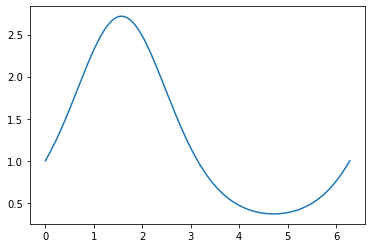
\includegraphics[scale=1]{In Progress/output_3_0.png}
\end{center}

\begin{align*}
    \text{Blue (obscured): } & f(x) 
    & \text{Red: } & (x_j, f_j) \text{ for } j = 0, \dots, 7 
    & \text{Orange: } & P_8(x)
\end{align*}
\begin{center}
    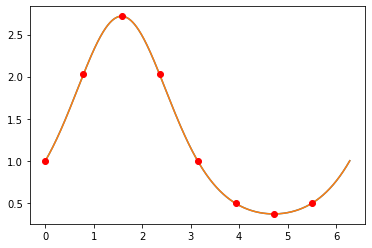
\includegraphics[scale=1]{In Progress/output_3_1.png}
\end{center}

\newpage

The trigonometric interpolating polynomial $P_N(x)$ is given by
\[
    P_N(x) = \frac12 a_0 + \sum_{k=1}^{N/2-1} (a_k \cos kx + b_k \sin kx) + \frac12 a_{N/2} \cos \left( \frac{N}{2} x \right).
\]
Differentiating with respect to $x$, we obtain
\begin{align*}
    P_N'(x)
        &= \sum_{k=1}^{N/2-1} (-k a_k \sin kx + k b_k \cos kx) - N a_{N/2} \sin \left( \frac{N}{2} x \right) \\
        &= \sum_{k=1}^{N/2-1} k(b_k \cos kx - a_k \sin kx) - N a_{N/2} \sin \left( \frac{N}{2} x \right).
\end{align*}
Using the same method as above, we compute the lists of coefficients of $P_N(x)$, then implement the above formula for the derivative of $P_N(x)$ to plot the result.
\begin{lstlisting}[language=Python]
def dP(N, A, B, x):
    return sum([k*(B[k]*cos(k*x) - A[k]*sin(k*x)) \
                   for k in range(1, int(N/2))]) \
            + N*A[-1]*sin(N/2*x)

def main_3b():
    N = 8
    X = [j*2*pi/N for j in range(0, N)]
    F = [exp(sin(x)) for x in X]
    
    C = rfft(F)
    A = 2/N * C.real
    B = -2/N * C.imag
    
    M = 1000
    X_dom = [2*pi*l/M for l in range(0, M+1)]
    dF_val = [cos(x)*exp(sin(x)) for x in X_dom]
    dP_val = [dP(N, A, B, x) for x in X_dom]
    
    plt.plot(X_dom, dF_val)
    plt.plot(X_dom, dP_val)
    plt.show()
    
    for x in X:
        print(dP(N, A, B, x), cos(x)*exp(sin(x)) - dP(N, A, B, x))
    
main_3b()
\end{lstlisting}

\newpage

\begin{align*}
    \text{Blue: } & f'(x) = e^{\sin x}\cos x & \text{Orange: } & P_8'(x)
\end{align*}
\begin{center}
    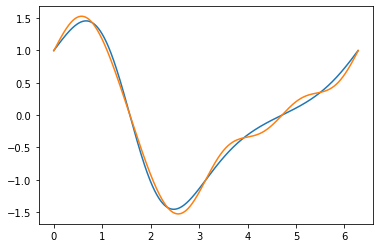
\includegraphics[scale=1]{In Progress/output_5_0.png}
\end{center}

Note that $P_8'$ is not a trigonometric interpolating polynomial of $f'$. Rather, it is the derivative of $P_8$, the trigonometric interpolating polynomial of $f$. The points where $P_8'$ intersects $f'$ are very close to the nodes where $P_8$ interpolates $f$, but the table below shows us that $P_8'$ does not interpolate $f'$ at these points. (That being said, the computed value and error of $P_8'$ at $x_2$ and $x_6$ is very close to zero, which is the value of $f'$ at these points. I would wager a guess that the actual value of $P_8'$ is exact at these points, but I did not prove this.)

\[\begin{array}{c|l|l}
    j & P_8'(x_j) & \text{Error} \\
    \hline
    0 & \phantom{-}0.9956     & \phantom{-}0.0043 \\
    1 & \phantom{-}1.4375      & -0.0034 \\
    2 & \phantom{-}2.7978\times10^{-17}   & \phantom{-}1.3846\times10^{-16} \\
    3 & -1.4375     & \phantom{-}0.0034 \\
    4 & -0.9956    & -0.0043 \\
    5 & -0.3513     & \phantom{-}0.0027 \\
    6 & -3.5646\times10^{-17} & -3.1931\times10^{-17} \\
    7 & \phantom{-}0.3513     & -0.0027
\end{array}\]



\newpage
\section{}
\begin{problem}
    The solution $P_n(x)$ to the Least Squares Approximation problem of $f$ by a polynomial of degree at most $n$ is given explicitly in terms of orthogonal polynomial $\psi_0(x), \psi_1(x), \dots, \psi_n(x)$, where $\psi_j$ is a polynomial of degree $j$, by
    \[
        P_n(x) = \sum_{j=0}^n a_j \psi_j(x), \quad a_j = \frac{\< f, \psi_j \>}{\< \psi_j, \psi_j \>}.
    \]
\end{problem}

\subsection{}
\begin{problem}
    Let $\PP_n$ be the space of polynomials of degree at most $n$. Prove that the error $f - P_n$ is orthogonal to this space, i.e. $\< f - P_n, q \> = 0$ for any $q \in \PP_n$.
\end{problem}


\begin{proof}
    Let $q \in \PP_n$. Since $\psi_0, \dots, \psi_n$ are linearly independent and the dimension of $\PP_n$ is $n+1$, then they form a basis. So $q$ can be written as a linear combination of these polynomials,
    \[
        q = \sum_{j=0}^n b_j \psi_k.
    \]
    Now by the linearity of the inner product we find
    \[
        \<f - P_n, q\> = \<f, q\> - \<P_n, q\>.
    \]
    Then
    \[
        \<f, q\> = \<f, b_0\psi_0 + \cdots + b_n\psi_n\> = \sum_{j=0}^n b_j \<f, \psi_j\>
    \]
    and
    \[
        \<P_n, q\>
            = \<a_0\psi_0 + \cdots + a_n\psi_n,\; b_0\psi_0 + \cdots + b_n\psi_n\> \\
            = \sum_{j=0}^n \sum_{k=0}^n a_j b_k \<\psi_j, \psi_k\>.
    \]
    Now since $\psi_0, \dots, \psi_n$ are orthogonal, we have
    \[
        \<P_n, q\> = \sum_{j=0}^n \sum_{k=0}^n a_j b_k \<\psi_j, \psi_k\>\delta_{j,k} = \sum_{j=0}^n a_j b_j \<\psi_j, \psi_j\>
    \]
    Finally, the definition of $a_j$ gives us
    \[
        \<f - P_n, q\> = \sum_{j=0}^n b_j(\<f, \psi_j\> - a_j\<\psi_j, \psi_j\>) = \sum_{j=0}^n b_j(0) = 0.
    \]
    
\end{proof}

\newpage
\subsection{}
\begin{problem}
    Using the analogy of vectors interpret this result geometrically (recall the concept of orthogonal projection).
\end{problem}
\medskip

The space $\PP_n$ of polynomials of degree at most $n$ is a vector space where the vectors are functions. It is a subspace of the larger vector space of functions on which our inner product is defined, i.e., the inner product space. Any inner product space is the orthogonal sum of a subspace and its orthogonal complement. In particular, our inner product space is the orthogonal sum of $\PP_n$ and it orthogonal complement. Now any vector $v$ in the inner product space can be written as $v = x + y$ where $x \in \PP_n$ and $y \in \PP_n^\perp$. In particular, $x \perp y$ and we say that $x$ is the orthogonal projection of $v$ onto $\PP_n$, written $x = \operatorname{proj}_{\PP_n} v$. Then, we have the difference $v - \operatorname{proj}_{\PP_n} v = y \in \PP_n^\perp$.

When we have an orthogonal basis of a subspace, as we do with $\psi_0,\dots,\psi_n$ for $\PP_n$, then the orthogonal projection is given simply in terms of the inner products with the basis vectors. In particular, taking $f \in \PP_n$ as above, then $P_n$ is precisely the orthogonal projection of $f$ onto $\PP_n$. And we obtain
\[
    f - P_n = f - \operatorname{proj}_{\PP_n} f \in \PP_n^\perp,
\]
which is to say that $f - P_n$ is orthogonal to everything in $\PP_n$.


\newpage
\section{}

\subsection{}
\begin{problem}
    Obtain the first $4$ Legendre polynomials in $[-1, 1]$.
\end{problem}
\medskip

We use the inner product
\[
    \<u, v\> = \int_{-1}^1 u(x) v(x) \,dx
\]
on the linearly independent set of polynomials $\{1, x, x^2, x^3\}$ to produce a set of orthogonal polynomials $\{\psi_0, \psi_1, \psi_2, \psi_3\}$. We take $\psi_0 = 1$, then $\psi_1$ is given by
\[
    \psi_1 = x - \proj_{\psi_0} x.
\]
We find
\[
    \proj_{\psi_0} x 
        = \psi_0 \cdot \frac{\< x, \psi_0\>}{\<\psi_0, \psi_0\>}
        = 1 \cdot \frac{\int_{-1}^1 x \,dx}{\int_{-1}^1 \,dx}
        = \frac{\frac12 x^2 \big|_{-1}^1}{x \big|_{-1}^1}
        = \frac{0}{2}
        = 0.
\]
Thus, $\psi_1 = x$. Next, $\psi_2$ is given by
\[
    \psi_2 = x^2 - \proj_{\psi_1} x^2 - \proj_{\psi_0} x^2.
\]
We find
\[
    \proj_{\psi_1} x^2 
        = \psi_1 \cdot \frac{\< x^2, \psi_1\>}{\<\psi_1, \psi_1\>}
        = x \cdot \frac{\int_{-1}^1 x^3 \,dx}{\int_{-1}^1 x^2 \,dx}
        = x \cdot \frac{\frac14 x^4 \big|_{-1}^1}{\frac13 x^3 \big|_{-1}^1}
        = x \cdot \frac{0}{\frac23}
        = 0,
\]
and
\[
    \proj_{\psi_0} x^2 
        = \psi_0 \cdot \frac{\< x^2, \psi_0\>}{\<\psi_0, \psi_0\>}
        = 1 \cdot \frac{\int_{-1}^1 x^2 \,dx}{2}
        = \frac{\frac23}{2}
        = \frac13.
\]
Thus, $\psi_2 = x^2 - \frac13$. Finally, $\psi_3$ is given by
\[
    \psi_2 = x^3 - \proj_{\psi_2} x^3 - \proj_{\psi_1} x^3 - \proj_{\psi_0} x^3.
\]
We find
\begin{align*}
    \proj_{\psi_2} x^3 
        &= \psi_2 \cdot \frac{\< x^3, \psi_2\>}{\<\psi_2, \psi_2\>} \\
        &= (x^2 - \tfrac13) \cdot \frac{\int_{-1}^1 (x^5 - \frac13 x^3) \,dx}{\int_{-1}^1 (x^4 - \frac23 x^2 + \frac19) \,dx} \\
        &= (x^2 - \tfrac13)  \cdot \frac{\frac16 x^6 - \frac1{12} x^4 \big|_{-1}^1}{\frac15 x^5 - \frac29 x^3 + \frac19 x \big|_{-1}^1} \\
        &= (x^2 - \tfrac13)  \cdot \frac{0}{\frac8{45}} \\
        &= 0,
\end{align*}
\[
    \proj_{\psi_1} x^3 
        = \psi_1 \cdot \frac{\< x^3, \psi_1\>}{\<\psi_1, \psi_1\>}
        = x \cdot \frac{\int_{-1}^1 x^4 \,dx}{\frac23}
        = x \cdot \frac{\frac15 x^5 \big|_{-1}^1}{\frac23}
        = x \cdot \frac{\frac25}{\frac23}
        = \tfrac35 x,
\]
and
\[
    \proj_{\psi_0} x^3 
        = \psi_0 \cdot \frac{\< x^3, \psi_0\>}{\<\psi_0, \psi_0\>}
        = 1 \cdot \frac{\int_{-1}^1 x^3 \,dx}{2}
        = \frac{0}{2}
        = 0.
\]
Thus, $\psi_3 = x^3 - \frac35 x$. And we have the set of four orthogonal polynomials
\[
    \{1,\; x,\; x^2 - \tfrac13,\; x^3 - \tfrac35x\}.
\]


\subsection{}
\begin{problem}
    Find the least squares polynomial approximations of degrees $1$, $2$, and $3$ for the function $f(x) = e^x$ on $[-1, 1]$.
\end{problem}
\medskip

We take the Legendre polynomials, as derived in Problem 5(a), as an orthogonal basis for the space of polynomials $\PP_n$. The least squares polynomial approximation of $e^x$ of degree $n$ is given by
\[
    P_n = \sum_{j=0}^n a_j \psi_j,
\]
where
\[
    a_j =  \frac{\< e^x, \psi_j\>}{\<\psi_j, \psi_j\>},
\]
and the inner product is defined as above. We now find
\[
    a_0 = \frac{\int_{-1}^1 e^x \,dx}{\int_{-1}^1 \,dx} \approx \frac{2.3504}{2} = 1.1752,
\]\\
\[
    a_1 = \frac{\int_{-1}^1 xe^x \,dx}{\int_{-1}^1 x^2 \,dx} \approx \frac{0.7358}{0.6667} \approx 1.1036,
\]\\
\[
    a_2 = \frac{\int_{-1}^1 (x^2 - \frac13)e^x \,dx}{\int_{-1}^1 (x^2 - \frac13)^2 \,dx} \approx \frac{0.0953}{1.7778} \approx 0.5367,
\]\\
\[
    a_3 = \frac{\int_{-1}^1 (x^3 - \tfrac35x)e^x \,dx}{\int_{-1}^1 (x^3 - \tfrac35x)^2 \,dx} \approx \frac{0.0081}{0.0457} \approx 0.1772.
\]
And we obtain the least squares polynomial approximations of $e^x$
\[
    P_1 = a_0 + a_1x \approx 1.1752 + 1.1036x,
\]\\
\[
    P_2 = P_1 + a_2(x^2 - \tfrac13) \approx 0.9963 + 1.1036x + 0.5367x^2,
\]\\
\[
    P_3 = P_2 + a_3(x^3 - \tfrac35x) \approx 0.9963 - 0.9973x + 0.5367x^2 + 0.1772x^3.
\]



\subsection{}
\begin{problem}
    What is the polynomial least squares approximation of degree $4$ for $f(x) = x^3$ on $[-1, 1]$? Explain.
\end{problem}
\medskip

Since $x^3$ is a polynomial of degree $3$, then it is contained in the space $\PP_4$. Therefore, it can be represented exactly as a linear combination of the basis polynomials. In particular,
\[
    P_4 = 0\psi_0 + \frac35 \psi_1 + 0\psi_2 + \psi_3 + 0\psi_4 = \frac35x + x^3 - \frac35x = x^3.
\]
Since this approximation is exact, then the error is zero,
\[
    \|P_4 - x_3\| = \|x^3 - x^3\| = \|0\| = 0.
\]



\end{document}